\documentclass[a4paper]{article}

% Basic packages
\usepackage[fontset=fandol]{ctex}
\usepackage{amsmath, amssymb}
\usepackage{graphicx}
\usepackage[margin=2.5cm]{geometry}
\usepackage[most]{tcolorbox}
\usepackage{etoolbox}
\usepackage{listings}
\usepackage{hyperref}
\usepackage{booktabs}
\usepackage{subcaption}
\usepackage{float}
\usepackage{tikz}
\IfFileExists{pgfplots.sty}{
    \usepackage{pgfplots}
    \pgfplotsset{compat=1.18}
}{}

% Highlight boxes
\newtcolorbox{knowledgebox}[1]{
    enhanced, colback=blue!5!white, colframe=blue!75!black, colbacktitle=blue!75!black,
    coltitle=white, fonttitle=\bfseries, title=#1, attach boxed title to top left={yshift=-2mm, xshift=2mm},
    boxrule=1pt, sharp corners
}

\newtcolorbox{importantbox}[1]{
    enhanced, colback=yellow!10!white, colframe=yellow!80!black, colbacktitle=yellow!80!black,
    coltitle=black, fonttitle=\bfseries, title=#1, sharp corners
}

\newtcolorbox{warningbox}[1]{
    enhanced, colback=red!5!white, colframe=red!75!black, colbacktitle=red!75!black,
    coltitle=white, fonttitle=\bfseries, title=#1, sharp corners
}

% Listings
\lstset{
    language=Python,
    basicstyle=\ttfamily\small,
    keywordstyle=\color{blue},
    stringstyle=\color{red!60!black},
    commentstyle=\color{green!60!black},
    breaklines=true,
    frame=single,
    numbers=left,
    numberstyle=\tiny\color{gray},
    captionpos=b,
    extendedchars=false
}

% Front-page metadata
\newcommand{\notetitle}{Lecture 5A: 机器人动力学、控制与运动规划}
\newcommand{\noteauthors}{五道口纳什 \& Codex}
\newcommand{\notedate}{\today}
\newcommand{\videochannel}{UC Berkeley CS294-277 / Jitendra Malik}
\newcommand{\videopublishdate}{2024-10-07}
\newcommand{\videoduration}{未记录}
\newcommand{\videourl}{https://www.youtube.com/watch?v=p8ZALhlrBrI}
\newcommand{\videocoverpath}{cover.jpg}

\begin{document}

\begin{titlepage}
\centering
{\Large 课程笔记\par}
\vspace{1.2cm}
{\huge\bfseries \notetitle\par}
\vspace{0.8cm}
{\large \noteauthors\par}
\vspace{0.3cm}
{\large \notedate\par}
\vspace{1.2cm}

\ifdefempty{\videocoverpath}{
{\small 请在生成笔记时填入视频封面图的本地路径。\par}
}{
\includegraphics[width=0.82\textwidth,height=0.45\textheight,keepaspectratio]{\videocoverpath}\par
}

\vfill
\begin{tcolorbox}[width=0.9\textwidth, colback=black!2!white, colframe=black!60, sharp corners]
\textbf{视频作者/频道}：\videochannel\par
\textbf{发布日期}：\videopublishdate\par
\textbf{视频时长}：\videoduration\par
\textbf{视频链接}：
\ifdefempty{\videourl}{
未填写
}{
\href{\videourl}{\nolinkurl{\videourl}}
}
\end{tcolorbox}
\end{titlepage}

\tableofcontents
\newpage

\begin{figure}[H]
\centering
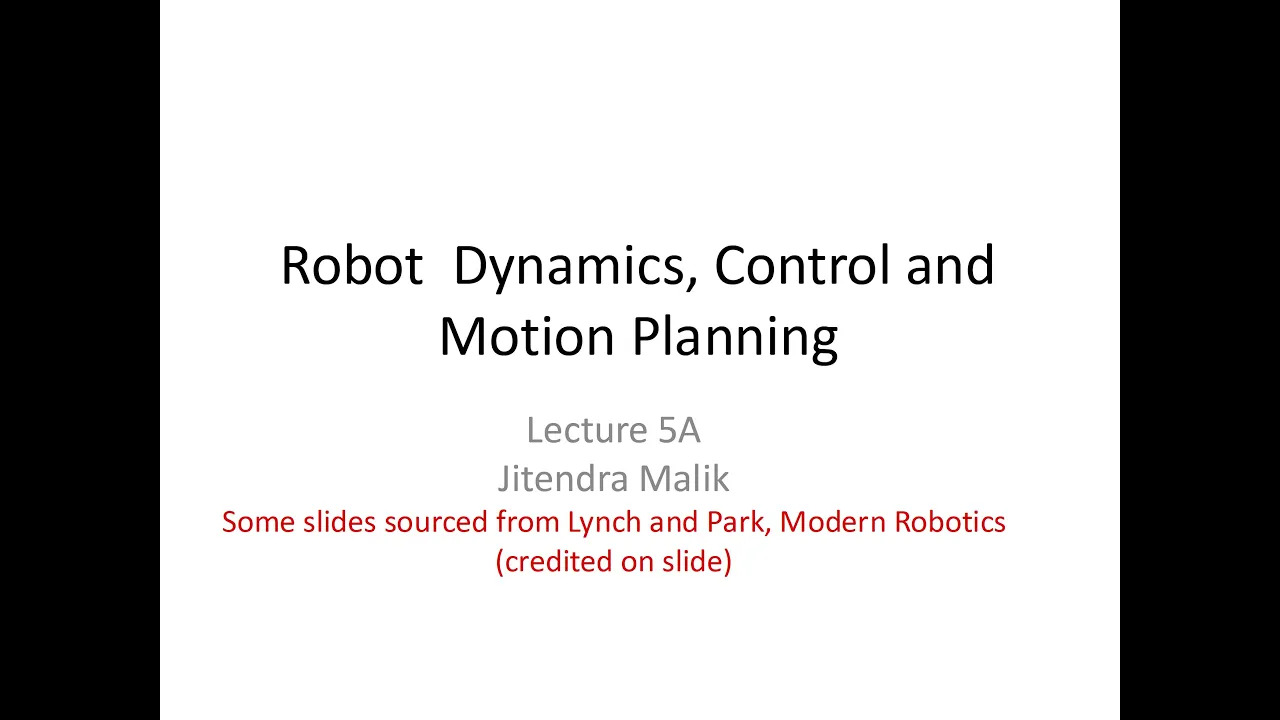
\includegraphics[width=0.78\textwidth]{overview_cover.jpg}
\caption{课程官方材料中的代表性页面，用于帮助读者在进入本讲正文前建立整体上下文。}
\end{figure}
\section{机器人动力学：从位姿到受力}
这一讲的前三分之一实际上是在把经典机器人学的语言重新铺平：先说运动学，再说动力学，最后才进入控制和规划。讲者明确提醒，动力学、控制和运动规划并不是彼此孤立的主题，而是同一个机器人系统在不同抽象层上的描述。

\subsection{正运动学与连杆建模}
正运动学（forward kinematics）回答的是：已知各关节变量，末端执行器的位置和姿态是什么。对于串联机械臂，课程页给出了 product of exponentials（PoE）公式：

\[
T = e^{\hat{\xi}_1 \theta_1} e^{\hat{\xi}_2 \theta_2} \cdots e^{\hat{\xi}_n \theta_n} T_0
\]

这里，\(T\) 是末端位姿，\(T_0\) 是零位形时的末端位姿，\(\hat{\xi}_i\) 表示第 \(i\) 个关节的螺旋轴（screw axis）的李代数表示，\(\theta_i\) 是关节角。讲者把这个公式作为“把几何写成代数”的典型例子，因为它让运动学可以直接接入控制和优化。

\begin{knowledgebox}{URDF}
URDF（Unified Robot Description Format）是描述机器人结构的 XML 格式，既记录关节运动学，也记录连杆的质量、惯量和几何。它本质上把“机器人是什么”写成一棵树。
\end{knowledgebox}

课程页用 URDF 片段强调两类元素：joint element 负责运动学，link element 负责惯性参数。这个区分很重要，因为后续动力学公式里的质量矩阵、重力项和科氏项都依赖这些结构化参数。

\subsection{正逆动力学}
正动力学（forward dynamics）和逆动力学（inverse dynamics）是一对互逆问题。前者输入力矩，求加速度；后者输入期望加速度，求需要施加的力矩。

\[
\ddot q = f(\tau, q, \dot q)
\]

\[
\tau = M(q)\ddot q + C(q,\dot q)\dot q + g(q)
\]

其中，\(\tau\) 是关节力矩，\(q\) 是关节位置，\(\dot q\) 是关节速度，\(\ddot q\) 是关节加速度，\(M(q)\) 是质量矩阵，\(C(q,\dot q)\) 是速度相关项，\(g(q)\) 是重力项。讲者进一步提醒，动力学通常有两种等价推导路线：Lagrangian dynamics（基于能量和变分原理）与 Newton-Euler dynamics（基于刚体受力平衡）。

\begin{importantbox}{为什么要看动力学}
只看运动学，机器人像一个“几何对象”；加上动力学之后，机器人才真正变成一个“会受力、会加速、会被扰动”的物理系统。控制设计如果忽略这一步，后面就很难解释为什么 feedforward 和 feedback 必须结合。
\end{importantbox}

\subsection{本章小结}
动力学部分的核心不是记公式，而是理解机器人模型的层级：几何由运动学给出，物理由动力学给出，控制则是在动力学模型之上写出期望行为。PoE、URDF 和逆动力学公式构成了这套语言的基础。

\section{控制：从巡航控制到 PID}
控制部分从一个非常朴素的巡航控制（cruise control）例子开始。这个选择并不随意，因为它能把 feedforward 与 feedback 的差别讲得极其清楚。

\subsection{开环与闭环}
在开环控制（open-loop control，也就是 feedforward control）里，控制器只根据目标输入发命令，不看输出误差。课程页里的模型说明了坡度扰动 \(w\) 会如何影响速度 \(y\)：

\[
y = 10(u - 0.5w), \qquad y = r - 5w
\]

如果道路坡度变化没有被显式补偿，系统就会偏离参考速度 \(r\)。相反，在闭环控制（closed-loop control，也就是 feedback control）里，控制器根据误差 \(r-y\) 不断修正输入：

\[
u = 10(r-y)
\]

代回模型后，扰动项的影响显著被压低。课程页用“reduced by 100x”这类直观表述来说明，闭环不是为了替代物理模型，而是为了在模型不完美时兜底。

\subsection{PID 控制}
PID（Proportional-Integral-Derivative）控制是机器人与自动化里最经典的控制律之一：

\[
u(t) = K_p e(t) + K_i \int_0^t e(\tau)\,d\tau + K_d \frac{de(t)}{dt}
\]

这里，\(K_p\) 负责当前误差，\(K_i\) 累积历史误差，\(K_d\) 观察误差变化趋势。课程页还用 motion control 的误差响应来强调三个性能指标：steady-state error、overshoot 和 settling time。也就是说，PID 不只是“能用”，而是把响应速度、稳定性和精度放在同一个调参框架里。

\subsection{运动控制、力控制与混合控制}
讲者把控制目标进一步分成 motion control、force control、hybrid motion-force control 和 impedance control。这个分类非常实用，因为它逼着我们先问“任务要求控制什么”，再问“控制器该怎么写”。

\begin{itemize}
  \item 运动控制（motion control）：跟踪轨迹或位姿。
  \item 力控制（force control）：维持接触力，避免过压或失稳。
  \item 混合控制（hybrid control）：某些方向控位置，某些方向控力。
  \item 阻抗控制（impedance control）：不直接追求刚性位置，而是调节系统对外力的响应方式。
\end{itemize}

课程页列了很多任务，比如 shaking hands、erasing a whiteboard、spray painting、inserting a peg in a hole、polishing、folding laundry。它们的共同点是：一旦机器人和环境发生持续接触，单纯的位姿跟踪就不够了，必须考虑接触力、柔顺性和任务阶段切换。

\subsection{反馈线性化与计算力矩}
在讲到动力学与控制的连接时，课程末尾提到了 computed torque control，也就是 feedback linearization 的一类典型形式。这里的关键思路是：前馈部分负责补偿已知动力学，反馈部分负责处理建模误差和扰动。讲者虽然没有把这部分展开成完整推导，但它与前面的 cruise control 例子在思想上完全一致。

\subsection{本章小结}
控制部分传达的最重要信息是：没有一种控制器能在所有任务上独立工作。开环依赖模型，闭环依赖观测，PID 把误差动态组织起来，而 force control / impedance control 则把接触任务纳入控制目标。真正可用的系统通常是前馈和反馈的组合。

\section{运动规划：C-space、PRM 与时间缩放}
这一部分把注意力从“控制怎么稳”转向“怎么走过去”。如果说控制决定的是“怎么把轨迹执行出来”，那 motion planning 决定的是“轨迹本身怎么被找出来”。

\subsection{路径、轨迹与时间缩放}
课程页明确区分了 path 和 trajectory：

\begin{itemize}
  \item Path：只描述构型随路径参数变化的曲线。
  \item Trajectory：把路径嵌入时间，描述构型随时间变化。
  \item Time scaling：给路径参数加上 \(s(t)\)，把空间曲线变成时间曲线。
\end{itemize}

讲者强调，轨迹不只是“多了一个时间轴”，它还包含平滑性要求。S-curve time scaling 的意义就在于让速度和加速度逐步变化，避免突然的 jerk。对于抓取、接近、放置这类任务，平滑的时间缩放比简单的线性插值更符合物理约束。

\subsection{配置空间与障碍膨胀}
motion planning 的标准做法是在配置空间（configuration space, C-space）中规划，而不是在笛卡尔空间里直接“画线”。课程页通过两个概念把这个问题说清楚：

\begin{itemize}
  \item \(C_{\mathrm{free}}\)：不碰撞的配置集合。
  \item \(C_{\mathrm{obs}}\)：发生碰撞的配置集合。
\end{itemize}

对于非点机器人，课程页提出一种常见处理：不是把机器人“缩成点”，而是把障碍物按机器人半径进行膨胀（grow obstacles）。这样可以把碰撞检测转化成点机器人问题。这个技巧很重要，因为它把复杂几何问题变成了更容易处理的保守近似。

\subsection{PRM：概率路网}
Probabilistic Roadmap（PRM）是这一讲最核心的规划算法。它先离线构建 road map，再在查询时快速找路，因此很适合重复查询的场景。课程页的算法可以概括为：

\begin{lstlisting}[caption={PRM 的构建与查询逻辑（教学性伪代码）}]
for i = 1..N:
    sample qi from C_free
    add qi to roadmap R

for each qi in R:
    N(qi) <- k nearest neighbors of qi
    for each q in N(qi):
        if local path from q to qi is collision-free:
            add edge (q, qi) to R

query(start, goal):
    connect start and goal to nearby roadmap nodes
    search shortest path on R
\end{lstlisting}

这段伪代码背后的思想很简单：把“连续的几何规划”变成“图搜索”。构建路网的成本可以提前支付，在线阶段只需要找最近节点并做最短路搜索。讲者同时提到 RRT 和 RRT*，它们是在不需要复用同一条 roadmap 时更合适的替代方案。

\subsection{为什么经典规划仍然不够}
讲者在这里埋了一个和下一讲相连的伏笔：经典 motion planning 的前提是环境被完全知道，但现实中障碍信息来自感知系统，而感知本身是有噪声、延迟和局部性的。也就是说，规划问题不再只是“给定地图找路”，而是“在不完整感知下持续更新地图并做局部回退”。

\subsection{本章小结}
这一讲把 classical robotics 的三件事串起来了：动力学告诉我们机器人如何受力，控制告诉我们如何把误差压下去，运动规划告诉我们如何在障碍物之间找到可执行的路径。PRM 和 C-space 是其中最具代表性的抽象，而 time scaling 则把几何路径变成可执行轨迹。

\section{总结与延伸}
这讲是后续课程的基础层。没有正逆动力学，就很难理解 computed torque control；没有 C-space 和 PRM，就很难理解后面关于规划与预测的讨论；没有 path / trajectory 的区分，就很难把“能到达”与“能平滑到达”分开。换句话说，这一讲不是在做历史回顾，而是在建立后面所有机器人系统都要用到的语法。

如果继续往后看，最值得延伸的方向有两个：一是把 classical control 和 learning-based policy 结合起来，看看 feedforward 与 feedback 如何在数据驱动系统里重新出现；二是把 motion planning 和 perception 结合起来，思考在不完美观测下如何在线更新 C-space。后面 5B 的内部模型和预测控制，正是对这个问题的进一步回答。

\end{document}
